\section{Group -- Plant-Condenser Control}\label{group-plant-condenser-control}

\subsection{Operation Schemes (Plant and Condenser)}\label{operation-schemes-plant-and-condenser}

Plants and condenser loops must have some mechanism for controlling the operation of the loop and which equipment is available under what conditions. Since there may be multiple control schemes that are assigned various priorities associated with each loop, an overall operation scheme must be defined. The overall scheme consists of the object name, an identifying name that is referenced in the main plant or condenser loop statement, and a list of operation schemes. Each operation scheme must have the type of operation scheme, its identifying name, and the schedule that defines its availability. Note that the order in which the individual operation schemes appear in this list defines its priority versus the others with the same scheduled availability. The first scheme appearing in the list is given the highest priority, the second scheme has second highest priority, etc. In other words, if according to its schedule, the first operation scheme is available, then it is used by the simulation to define how the plant or condenser loop operates. If it is not available, the second operation scheme in the list is checked to see if it is available until the highest priority scheme that is also available is found.~ To allow for simultaneous heating and cooling, there is one configuration where multiple operation schemes are available at a given timestep.~ This is allowed if a user inputs both a heating range based operation and a cooling range based operation with overlapping schedules.~ The simulation will look at the current loop demand to determine if the cooling scheme should be used or the heating scheme.~ In other cases, if two schemes overlap (are available at the same time), a fatal error will be encountered.

\subsection{PlantEquipmentOperationSchemes}\label{plantequipmentoperationschemes}

\subsubsection{Inputs}\label{inputs-033}

\paragraph{Field: Name}\label{field-name-032}

This alpha field contains the identifying name given to the Plant Operation Scheme. This name is placed in the Plant Loop object to select this scheme.

\paragraph{Field Set: (Component Object Type, Name, Schedule) up to 8}\label{field-set-component-object-type-name-schedule-up-to-8}

Operation schemes are listed in ``priority'' order.~ Note that each scheme must address the entire load and/or condition ranges for the simulation. The actual one selected for use will be the first that is ``Scheduled'' on.~ That is, if control scheme 1 is not ``on'' and control scheme 2 is -- then control scheme 2 is selected. Only plant equipment should be listed on a Control Scheme for this item.

\paragraph{Field: Control Scheme \textless{}\#\textgreater{} Object Type}\label{field-control-scheme-object-type}

This alpha field contains the keyword for the type of control scheme used. The options for plant control schemes are:

\begin{itemize}
\item
  \hyperref[plantequipmentoperationuncontrolled]{PlantEquipmentOperation:Uncontrolled}
\item
  \hyperref[plantequipmentoperationcoolingload]{PlantEquipmentOperation:CoolingLoad}
\item
  \hyperref[plantequipmentoperationheatingload]{PlantEquipmentOperation:HeatingLoad}
\item
  \hyperref[plantequipmentoperationoutdoordrybulb]{PlantEquipmentOperation:OutdoorDryBulb}
\item
  \hyperref[plantequipmentoperationoutdoorwetbulb]{PlantEquipmentOperation:OutdoorWetBulb}
\item
  \hyperref[plantequipmentoperationoutdoorrelativehumidity]{PlantEquipmentOperation:OutdoorRelativeHumidity}
\item
  \hyperref[plantequipmentoperationoutdoordewpoint]{PlantEquipmentOperation:OutdoorDewpoint}
\item
  \hyperref[plantequipmentoperationoutdoordrybulbdifference]{PlantEquipmentOperation:OutdoorDryBulbDifference}
\item
  \hyperref[plantequipmentoperationoutdoorwetbulbdifference]{PlantEquipmentOperation:OutdoorWetBulbDifference}
\item
  \hyperref[plantequipmentoperationoutdoordewpointdifference]{PlantEquipmentOperation:OutdoorDewpointDifference}
\item
  \hyperref[plantequipmentoperationcomponentsetpoint]{PlantEquipmentOperation:ComponentSetpoint}
\item
  \hyperref[plantequipmentoperationthermalenergystorage]{PlantEquipmentOperation:ThermalEnergyStorage}
\item
  \hyperref[plantequipmentoperationuserdefined]{PlantEquipmentOperation:UserDefined}
\item
  \hyperref[plantequipmentoperationchillerheaterchangeover]{PlantEquipmentOperation:ChillerHeaterChangeover}
\end{itemize}

\paragraph{Field: Control Scheme \textless{}\#\textgreater{} Name}\label{field-control-scheme-name}

This alpha field contains the identifying name given to the control scheme. These must be the named versions of the referenced Control Scheme (e.g.. a Uncontrolled Loop Operation with this name or a Cooling or Heating Load Range Based Operation with this name).

\paragraph{Field: Control Scheme \textless{}\#\textgreater{} Schedule}\label{field-control-scheme-schedule}

This alpha field contains the schedule name for the control scheme. This schedule consists of weeks and days, with the days containing ``0 or 1'' for each hour of the day. This binary schedule (0 for off, 1 for on) determines if the control scheme is operating for that hour of day or not.

Examples of this statement in two different IDFs:

\begin{lstlisting}

PlantEquipmentOperationSchemes,
      CW Loop Operation,       !- Name
      PlantEquipmentOperation:CoolingLoad,  ! Control Scheme 1 Object Type
      Peak Operation,          !- Control Scheme 1 Name
      On Peak,                 !- Control Scheme 1 Schedule
      PlantEquipmentOperation:CoolingLoad,  ! Control Scheme 2 Object Type
      Off Peak Operation,      !- Control Scheme 2 Name
      Off Peak;                !- Control Scheme 2 Schedule

  PlantEquipmentOperationSchemes,
      CW Loop Operation,       !- Name
      PlantEquipmentOperation:CoolingLoad,  ! Control Scheme 1 Object Type
      Central Chiller Only,    !- Control Scheme 1 Name
      PlantOnSched;            !- Control Scheme 1 Schedule
\end{lstlisting}

In the first IDF example, ``\hyperref[plantequipmentoperationcoolingload]{PlantEquipmentOperation:CoolingLoad}'' is the type of control scheme. ``Peak Operation'' and ``Off Peak Operation'' are the names of two different load range based controls defined separately (see below -- ). ``On Peak'' and ``Off Peak'' are schedules defined elsewhere in the input file.

The load range based operation scheme has two statements associated with it: a main statement that defines the ranges that individual priority settings are valid and the lists of equipment that may be used for each range.

\subsection{CondenserEquipmentOperationSchemes}\label{condenserequipmentoperationschemes}

\subsubsection{Inputs}\label{inputs-1-030}

\paragraph{Field: Name}\label{field-name-1-029}

This alpha field contains the identifying name given to the Condenser Operation Scheme.

\paragraph{Field Set: (Component Object Type, Name, Schedule) up to 8}\label{field-set-component-object-type-name-schedule-up-to-8-1}

Operation schemes are listed in ``priority'' order.~ Note that each scheme must address the entire load and/or condition ranges for the simulation. The actual one selected for use will be the first that is ``Scheduled'' on.~ That is, if control scheme 1 is not ``on'' and control scheme 2 is -- then control scheme 2 is selected. Only condenser equipment should be listed on a Control Scheme for this item.

\paragraph{Field: Control Scheme \textless{}\#\textgreater{} Object Type}\label{field-control-scheme-object-type-1}

This alpha field contains the keyword for the type of control scheme used. The options for plant control schemes are:

This alpha field contains the keyword for the type of control scheme used. Currently, the available options are:

\begin{itemize}
\item
  \hyperref[plantequipmentoperationuncontrolled]{PlantEquipmentOperation:Uncontrolled}
\item
  \hyperref[plantequipmentoperationcoolingload]{PlantEquipmentOperation:CoolingLoad}
\item
  \hyperref[plantequipmentoperationheatingload]{PlantEquipmentOperation:HeatingLoad}
\item
  \hyperref[plantequipmentoperationoutdoordrybulb]{PlantEquipmentOperation:OutdoorDryBulb}
\item
  \hyperref[plantequipmentoperationoutdoorwetbulb]{PlantEquipmentOperation:OutdoorWetBulb}
\item
  \hyperref[plantequipmentoperationoutdoordewpoint]{PlantEquipmentOperation:OutdoorDewpoint}
\item
  \hyperref[plantequipmentoperationoutdoorrelativehumidity]{PlantEquipmentOperation:OutdoorRelativeHumidity}
\item
  \hyperref[plantequipmentoperationoutdoordrybulbdifference]{PlantEquipmentOperation:OutdoorDryBulbDifference}
\item
  \hyperref[plantequipmentoperationoutdoorwetbulbdifference]{PlantEquipmentOperation:OutdoorWetBulbDifference}
\item
  \hyperref[plantequipmentoperationoutdoordewpointdifference]{PlantEquipmentOperation:OutdoorDewpointDifference}
\item
  \hyperref[plantequipmentoperationuserdefined]{PlantEquipmentOperation:UserDefined}
\end{itemize}

The condenser operation schemes apply to the equipment on the `supply side' of the condenser loop---pumps, cooling towers, ground coupled heat exchangers, etc. The keywords select the algorithm that will be used to determine which equipment is available for each timestep. The Load Schemes schemes select a user specified set of equipment for each user specified range of a particular simulation variable. Load schemes compare the demand on the condenser supply side with specified load ranges and associated equipment lists. Outdoor schemes compare the current value of an environmental parameter with user specified ranges of that parameter.

\paragraph{Field: Control Scheme \textless{}\#\textgreater{} Name}\label{field-control-scheme-name-1}

This alpha field contains the identifying name given to the control scheme.

\paragraph{Field: Control Scheme \textless{}\#\textgreater{} Schedule}\label{field-control-scheme-schedule-1}

This alpha field contains the schedule name for the control scheme. This schedule consists of weeks and days, with the days containing ``0 or 1'' for each hour of the day. This binary schedule (0 for off, 1 for on) determines which control scheme is operating for a particular hour. The schedule facilitates daily or seasonal changes in control schemes to meet demand side management or energy conservation goals.

Scheduling conflicts are handled by selecting the first available scheme in order of appearance in the list.

Examples of this statement in two IDFs:

\begin{lstlisting}

CondenserEquipmentOperationSchemes,
      Tower Loop Operation,    !- CondenserOperationSchemeName
      PlantEquipmentOperation:CoolingLoad,  Control Scheme 1 Object Type
      Year Round Tower Operation,  !- Control Scheme 1 Name
      PlantOnSched;            !- Control Scheme 1 Schedule

  CondenserEquipmentOperationSchemes,Tower Loop Operation,
      PlantEquipmentOperation:CoolingLoad, Peak Load Operation, AFTERNOONSCHEDULE,
      PlantEquipmentOperation:CoolingLoad, OffPeak Load Operation, MORNINGSCHEDULE,
      PlantEquipmentOperation:OutdoorWetBulb, NightOperation, NIGHTSCHEDULE;
\end{lstlisting}

Each schedule (AFTERNOONSCHEDULE, MORNINGSCHEDULE, NIGHTSCHEDULE) invokes its associated operation scheme (Peak Load Operation, OffPeak Load Operation, NightOperation). The type of operation scheme and its name references the input syntax associated with the range specification and the associated equipment.

\subsection{PlantEquipmentOperation:Uncontrolled}\label{plantequipmentoperationuncontrolled}

Uncontrolled loop operation simply specifies a group of equipment that runs `uncontrolled'. If the loop runs, this equipment will run also, unless turned off by the loop flow resolver to maintain continuity in the fluid loop.

\subsubsection{Inputs}\label{inputs-2-028}

\paragraph{Field: Name}\label{field-name-2-027}

This alpha field contains the identifying name for the control scheme.

\paragraph{Field: Equipment List Name}\label{field-equipment-list-name}

This alpha field contains the identifying name for the Equipment List. This field ties to the Load Range Equipment List input structure, which must also be defined.

\paragraph{Field: Equipment List Name}\label{field-equipment-list-name-1}

This alpha field contains the identifying name for the Equipment List. This field ties to the \hyperref[plantequipmentlist]{PlantEquipmentList} or \hyperref[condenserequipmentlist]{CondenserEquipmentList} input structure, which must also be defined.

\subsection{PlantEquipmentOperation:CoolingLoad}\label{plantequipmentoperationcoolingload}

\subsubsection{Inputs}\label{inputs-3-025}

\subsection{PlantEquipmentOperation:HeatingLoad}\label{plantequipmentoperationheatingload}

The \hyperref[plantequipmentoperationcoolingload]{PlantEquipmentOperation:CoolingLoad} ~and PlantEquipmentOperation:HeatingLoad objects define the different ranges and which equipment list is valid for each range. After the keyword and the identifying name, a series of data trios is expected. In each trio, there is a lower limit for the load range, an upper limit for the load range, and a name that links to an equipment availability list (the \hyperref[plantequipmentlist]{PlantEquipmentList} or \hyperref[condenserequipmentlist]{CondenserEquipmentList} objects).

\subsubsection{Inputs}\label{inputs-4-022}

\paragraph{Field: Name}\label{field-name-3-022}

This alpha field contains the identifying name for the control scheme.

\paragraph{Field Set: (Lower limit, Upper Limit, Equip List name) up to 10}\label{field-set-lower-limit-upper-limit-equip-list-name-up-to-10}

\paragraph{Field: Load Range \textless{}\#\textgreater{} Lower Limit}\label{field-load-range-lower-limit}

This numeric field contains the lower demand range (W) for the equipment list. If demand is below this value, then this equipment list will not turn on to meet the demand.

\paragraph{Field: Load Range \textless{}\#\textgreater{} Upper Limit}\label{field-load-range-upper-limit}

This numeric field contains the upper demand range (W) for the equipment list. If demand is above this value, then this equipment list will not turn on to meet the demand.

\paragraph{Field: Range \textless{}\#\textgreater{} Equipment List Name}\label{field-range-equipment-list-name}

This alpha field contains the identifying name for the Equipment List (i.e., the name of a \hyperref[plantequipmentlist]{PlantEquipmentList} or \hyperref[condenserequipmentlist]{CondenserEquipmentList} object).

An example of these statements in an IDF is:

\begin{lstlisting}

PlantEquipmentOperation:CoolingLoad, Peak Operation,
          0,7000,   Chiller Plant,
          7000,24500,   Chiller Plant and Purchased,
          24500,500000, Purchased Only;
\end{lstlisting}

This particular load based operation scheme (above) has three different ranges. ``Chiller Plant'', ``Chiller Plant and Purchased'', and ``Purchased Only'' are names which link to various \hyperref[plantequipmentlist]{PlantEquipmentList} or \hyperref[condenserequipmentlist]{CondenserEquipmentList} objects as described below. Gaps may be left in the load ranges specified, but to operate equipment over the entire range the upper limit of a given range must equal the lower limit of the next range as shown in the example. If gaps are left in the load ranges specified, a warning message will be issued when the load to be met falls within a load range ``gap''. If the user wishes to leave a load range ``gap'' for a specific reason (no equipment to operate on this plant {[}or condenser{]} loop within this load range) and does not want the warning messages to be generated, then specify a lower limit, upper limit and equipment list name for the gap and do not specify any equipment in the associated equipment list, as shown below.

\begin{lstlisting}

PlantEquipmentOperation:CoolingLoad, Peak Operation,
      0,7000,   Chiller Plant,
      7000,7100, NoEquipmentOperationOnThisPlantLoop,
      7100,24500,   Chiller Plant and Purchased,
      24500,500000, Purchased Only;

  PlantEquipmentList,
      Chiller Plant,           !- Name
      Chiller:Electric,        !- Equipment 1 Object Type
      Big Chiller;             !- Equipment 1 Name

  PlantEquipmentList,
      NoEquipmentOperationOnThisPlantLoop;    !- Name

  PlantEquipmentList,
      Chiller Plant and Purchased,  !- Name
      Chiller:Electric,        !- Equipment 1 Object Type
      Big Chiller,             !- Equipment 1 Name
      DistrictCooling,         !- Equipment 2 Object Type
      Purchased Cooling;       !- Equipment 2 Name

  PlantEquipmentList,
      Purchased Only,          !- Name
      DistrictCooling,         !- Equipment 1 Object Type
      Purchased Cooling;       !- Equipment 1 Name
\end{lstlisting}

\subsection{PlantEquipmentOperation:OutdoorDryBulb}\label{plantequipmentoperationoutdoordrybulb}

\subsection{PlantEquipmentOperation:OutdoorWetBulb}\label{plantequipmentoperationoutdoorwetbulb}

\subsection{PlantEquipmentOperation:OutdoorRelativeHumidity}\label{plantequipmentoperationoutdoorrelativehumidity}

\subsection{PlantEquipmentOperation:OutdoorDewpoint}\label{plantequipmentoperationoutdoordewpoint}

The outdoor operation objects define the different ranges of the various environmental parameters and which equipment list is valid for each range. After the keyword and the identifying name, a series of data trios is expected. In each trio, there is a lower limit for the load range, an upper limit for the load range, and a name that links to an equipment availability list (the \hyperref[condenserequipmentlist]{CondenserEquipmentList}).

The fields for each of these are:

\subsubsection{Inputs}\label{inputs-8-015}

\paragraph{Field: Name}\label{field-name-4-019}

This alpha field contains the identifying name for the control scheme.

\paragraph{Field Set: (Lower limit, Upper Limit, Equip List name) up to 10}\label{field-set-lower-limit-upper-limit-equip-list-name-up-to-10-1}

\paragraph{Field: \textless{}specific type\textgreater{} Range \textless{}\#\textgreater{} Lower Limit}\label{field-specific-type-range-lower-limit}

This numeric field contains the lower limit (C for temperature operations, Percent for relative humidity operations) for the equipment list. If specific value is below this value, then this equipment list will not turn on to meet the demand.

\paragraph{Field: \textless{}specific type\textgreater{} Range \textless{}\#\textgreater{} Upper Limit}\label{field-specific-type-range-upper-limit}

This numeric field contains the lower limit (C for temperature operations, Percent for relative humidity operations) for the equipment list. If specific value is above this value, then this equipment list will not turn on to meet the demand.

\paragraph{Field: Range \textless{}\#\textgreater{} Equipment List Name}\label{field-range-equipment-list-name-1}

This alpha field contains the identifying name for the Equipment List (i.e., the name of a \hyperref[condenserequipmentlist]{CondenserEquipmentList} object).

\subsection{PlantEquipmentOperation:OutdoorDryBulbDifference}\label{plantequipmentoperationoutdoordrybulbdifference}

\subsubsection{Inputs}\label{inputs-9-013}

\subsection{PlantEquipmentOperation:OutdoorWetBulbDifference}\label{plantequipmentoperationoutdoorwetbulbdifference}

\subsubsection{Inputs}\label{inputs-10-012}

\subsection{PlantEquipmentOperation:OutdoorDewpointDifference}\label{plantequipmentoperationoutdoordewpointdifference}

The Delta Temperature based control strategies help to control any condenser equipment based on the difference between a reference node temperature and any environmental temperature. For example a cooling tower can be controlled by a strategy, which looks at the difference between the tower inlet temperature and wet-bulb temperature. A difference range is specified for each equipment list.

\subsubsection{Inputs}\label{inputs-11-011}

\paragraph{Field: Name}\label{field-name-5-016}

This alpha value contains the identifying name of the control strategy. This name appears as `control scheme name' in Condenser Operation Scheme object.

\paragraph{Field: Reference Temperature Node Name}\label{field-reference-temperature-node-name}

This alpha value specifies the reference node for the operation scheme identified in the first field.

\paragraph{Field Set: (Lower limit, Upper limit, Equipment List)}\label{field-set-lower-limit-upper-limit-equipment-list}

\paragraph{Field: \textless{}specific type\textgreater{} Range \textless{}\#\textgreater{} Lower Limit}\label{field-specific-type-range-lower-limit-1}

This numeric field specifies the minimum temperature difference required for the equipment specified in the equipment list to operate.

\paragraph{Field: \textless{}specific type\textgreater{} Range \textless{}\#\textgreater{} Upper Limit}\label{field-specific-type-range-upper-limit-1}

This numeric field specifies the maximum temperature difference below which the equipment specified in the equipment list is available.

\paragraph{Field: Range \textless{}\#\textgreater{} Equipment List Name}\label{field-range-equipment-list-name-2}

This alpha field contains the identifying name for the Equipment List (i.e., the name of a \hyperref[condenserequipmentlist]{CondenserEquipmentList} object).

\subsection{PlantEquipmentOperation:ComponentSetpoint}\label{plantequipmentoperationcomponentsetpoint}

In addition to load range based control on the plant loop, sequencing the plant components based on the outlet temperature of individual equipment is allowed. This scheme is common to many present-day Energy Management Systems sequencing. In this scheme, the sequencing is done based on the order specified in the control object described below.

However, when sequencing a boiler and a cooling tower to control the heating and cooling set point temperatures of a condenser loop, it is recommended that the boiler and the cooling tower be placed in a parallel configuration. The series configuration of these two equipment, though possible to model them, may result in simultaneous heating and cooling operation when the boiler is ON and the cooling tower operates in free cooling mode, i.e., 
the cooling tower may provide free cooling that could over cool the water below the boiler heating setpoint temperature.  


\subsubsection{Inputs}\label{inputs-12-011}

\paragraph{Field: Name}\label{field-name-6-014}

This field specifies the name of the operation scheme.

\paragraph{Field Set: Equipment Object Type, Name, Demand Calculation Node, Setpoint Node, Flow Rate, Operation Type)}\label{field-set-equipment-object-type-name-demand-calculation-node-setpoint-node-flow-rate-operation-type}

\paragraph{Field: Equipment \textless{}\#\textgreater{} Object Type}\label{field-equipment-object-type}

This field specifies the type of equipment controlled by scheme.

\paragraph{Field: Equipment \textless{}\#\textgreater{} Name}\label{field-equipment-name}

This field specifies the name of the controlled equipment.

\paragraph{Field: Demand Calculation \textless{}\#\textgreater{} Node Name}\label{field-demand-calculation-node-name}

The component demand will be calculated using the difference between the temperature at the demand node and the component set point temperature.

\paragraph{Field: Setpoint \textless{}\#\textgreater{} Node Name}\label{field-setpoint-node-name}

Each component controlled under temperature based control will have its own set point different from the loop set point. This field specifies component set point node (Generally its outlet temperatures). This node is acted upon by a SetpointManager in order to obtain the setpoint at any simulation timestep.

\paragraph{Field: Component \textless{}\#\textgreater{} Flow Rate}\label{field-component-flow-rate}

This numeric field specifies the design flow rate for the component specified in earlier fields. This flow rate is used to calculate the component demand. The field can be set to autosize, if the user wants the program to calculate the design flow. This would generally be set to autosize when the user does not know the component flow rate and does a sizing calculation for the corresponding component.

\paragraph{Field: Operation\textless{}\#\textgreater{} Type}\label{field-operation-type}

This alpha field specifies the operation mode for the equipment. The equipment can be in any of the three modes viz. Cooling, Heating and Dual. Dual is used when the components both as heating and cooling equipment (for example heat pumps).

And, as an example in an IDF:

\begin{lstlisting}

PlantEquipmentOperationSchemes,
      CW Loop Operation,       !- PlantOperationSchemeName
      PlantEquipmentOperation:ComponentSetpoint, ! Control Scheme 1 Object Type
      Test Scheme,                         !- Control Scheme 1 Name
      On;                                  !- Control Scheme 1 Schedule

  PlantEquipmentOperation:ComponentSetpoint,
      Test Scheme,
      CHILLER:ELECTRIC,        !- Equipment 1 Object Type
      Little Chiller,          !- Equipment 1 Name
      Little Chiller Inlet Node, !- Demand Calculation 1 Node Name
      Little Chiller Outlet Node, !- Setpoint 1 Node Name
      0.0011,                     !- Component 1 Flow Rate
      COOLING,                    !- Operation 1 Type
      CHILLER:ELECTRIC,        !- Equipment 2 Object Type
      Big Chiller,             !- Equipment 2 Name
      Big Chiller Inlet Node,  !- Demand Calculation 2 Node Name
      Big Chiller Outlet Node, !- Setpoint 2 Node Name
      0.0011,                  !- Component 2 Flow Rate
      COOLING;                 !- Operation 2 Type
\end{lstlisting}

\subsection{PlantEquipmentOperation:ThermalEnergyStorage}\label{plantequipmentoperationthermalenergystorage}

Users of thermal energy storage, particularly ice storage systems, are often faced with a challenge of specifying input for these systems. Essentially, they have to define various setpoint managers, temperature schedules, etc. in order to make the system functional. This plant/condenser control type simplifies the input somewhat by eliminating both a setpoint manager and a schedule for each piece of equipment that makes up the ice storage system. In fact, this operation scheme internally creates the setpoint managers required by the equipment listed as operated by the scheme defined by this syntax. While the more complex definition is possible and provides more flexibility like hourly variation of setpoint temperatures at the outlet of each piece of equipment, this input provides the most convenient method for making the system to work and assumes a single charging setpoint temperature and a single discharging setpoint temperature. For most systems, this is all that is needed.

\subsubsection{Inputs}\label{inputs-13-009}

\paragraph{Field: Name}\label{field-name-7-013}

This field defines the name of the thermal energy (ice) storage plant equipment operation scheme that will be referenced by the \hyperref[plantequipmentoperationschemes]{PlantEquipmentOperationSchemes} list in the plant input.

\paragraph{Field: On-Peak Schedule}\label{field-on-peak-schedule}

This field defines the name of an integer schedule that determines when on-peak electric pricing is in effect. This value is used to determine whether or not the ice storage system should be charging the ice storage unit. In the schedule, a value of 1 (or greater) corresponds to being in the on-peak period while any value of 0 or less corresponds to being in the off-peak period.

\paragraph{Field: Charging Availability Schedule}\label{field-charging-availability-schedule}

This field defines the name of an integer schedule that determines whether or not the system may enter charging mode off-peak. If the current value of the on-peak schedule is ``off'', then charging can take place if the charging availability schedule is ``on''. If the on-peak schedule is ``off'' and charging availability is ``off'', then charging is not allowed and the chiller and ice storage units controlled by this statement are operating to meet the non-charging chilled water temperature defined by the next input parameter. In this schedule, a value of 1 (or greater) corresponds to ``on'' when charging is available during an off-peak period while any value of 0 or less corresponds to chillers not being allowed to charge even during off-peak.

\paragraph{Field: Non-Charging Chilled Water Temperature}\label{field-non-charging-chilled-water-temperature}

This field defines the chilled water temperature when the ice storage system is NOT in charging mode. During these times, the storage system could be discharging or dormant depending on HVAC load conditions and ice storage controls. This value is used as the setpoint temperature for chillers associated with this plant equipment operation scheme during non-cooling season and during cooling season during the on-peak period. The cooling season and on-peak periods are defined by schedules reference to input above.

\paragraph{Field: Charging Chilled Water Temperature}\label{field-charging-chilled-water-temperature}

This field defines the chilled water temperature when the ice storage system is in charging mode. During these times, the chiller is producing a temperature low enough to generate ice in the ice storage unit. This value is used as the setpoint temperature for chillers associated with this plant equipment operation scheme during the cooling season during the off-peak period. The cooling season and on-peak periods are defined by schedules reference to input above.

\paragraph{Field Set: (Component Object Type, Name, Demand Calculation Node, Setpoint Node, Flow Rate, Operation Type)}\label{field-set-component-object-type-name-demand-calculation-node-setpoint-node-flow-rate-operation-type}

\paragraph{Field: Component \textless{}\#\textgreater{} Object Type}\label{field-component-object-type-001}

This field specifies the type of equipment controlled by scheme. This must be a thermal energy storage device (simple or detailed ice storage) or a chiller.

\paragraph{Field: Component \textless{}\#\textgreater{} Name}\label{field-component-name-002}

This field specifies the name of the controlled equipment. This name must be defined in the input as a valid ice storage device or chiller.

\paragraph{Field: Component \textless{}\#\textgreater{} Demand Calculation Node Name}\label{field-component-demand-calculation-node-name}

The component demand will be calculated using the difference between the temperature at the demand node and the component set point temperature.

\paragraph{Field: Component \textless{}\#\textgreater{} Setpoint Node Name}\label{field-component-setpoint-node-name}

Each component controlled under temperature based control will have its own set point different from the loop set point. This field specifies component set point node (Generally its outlet temperatures). This node is acted upon by a SetpointManager in order to obtain the setpoint at any simulation timestep.

\paragraph{Field: Component \textless{}\#\textgreater{} Flow Rate}\label{field-component-flow-rate-1}

This numeric field specifies the design flow rate for the component specified in earlier fields. This flow rate is used to calculate the component demand. The field can be set to autosize, if the user wants the program to calculate the design flow. This would generally be set to autosize when the user does not know the component flow rate and does a sizing calculation for the corresponding component.

\paragraph{Field: Component \textless{}\#\textgreater{} Operation Type}\label{field-component-operation-type}

This alpha field specifies the operation mode for the equipment. The equipment can be in any of the three modes viz. Cooling, Heating and Dual. Dual is used when the components both as heating and cooling equipment (for example heat pumps). Ice storage units can potentially either heat or cool the circulating fluid and thus should be defined as Dual mode.

An example IDF is shown below:

\begin{lstlisting}

PlantEquipmentOperationSchemes,
  CW Loop Operation,       !- Name
  PlantEquipmentOperation:ThermalEnergyStorage,  !- Control Scheme 1 Object Type
  Chiller and Partial Ice Storage,  !- Control Scheme 1 Name
  PlantOnSched;            !- Control Scheme 1 Schedule Name

  PlantEquipmentOperation:ThermalEnergyStorage,
  Chiller and Partial Ice Storage,  !- Name
  OnPeakEnergy,            !- On-Peak Schedule Name
  ChargingAvail,           !- Charging Availability Schedule Name
  7.22,                    !- Non-charging Chilled Water Temperature
  -5.0,                    !- Charging Chilled Water Temperature
  Chiller:Electric,        !- Component 1 Object Type
  Central Chiller,         !- Component 1 Name
  Central Chiller Inlet Node,  !- Component 1 Demand Calculation Node Name
  Central Chiller Outlet Node,  !- Component 1 Setpoint Node Name
  autosize,                !- Component 1 Flow Rate {m3/s}
  COOLING,                 !- Component 1 Operation Type
  ThermalStorage:Ice:Detailed,  !- Component 2 Object Type
  Ice Tank,                !- Component 2 Name
  Ice Tank Inlet Node,     !- Component 2 Demand Calculation Node Name
  Ice Tank Outlet Node,    !- Component 2 Setpoint Node Name
  0.13506E-02,             !- Component 2 Flow Rate {m3/s}
  DUAL;                    !- Component 2 Operation Type
\end{lstlisting}

\subsection{PlantEquipmentOperation:ChillerHeaterChangeover}\label{plantequipmentoperationchillerheaterchangeover}

Plant operation can difficult to control when air-to-water or water-to-water heat pumps are used as plant equipment.  Individual machines can be operated either as cooling or heat devices at any given time.  This object will poll the building to determine what type of loads are dominant and determine how the plant equipment should operate. Once the mode of operation is set the apparant plant loads are dispatched to equipment listed to meet those loads. For example, a heat pump capable of providing heating or cooling will be dispatched in heating mode. It is also possible to create a heat recovery heat pump connected between the heating and cooling plant loops where this heat pump can serve low loads on one plant while supplementing the operation of the other plant. Traditional plant controls cannot meet this type of equipment configuration. This object provides a supervisory controller can be used to control one heating and one cooling hydronic plant.

This object is used as a special plant operation scheme intended for a specific type of plant with both heating and cooling plant loops served by heat pumps which can switch between heating and cooling.  EnergyPlus's usual plant operation schemes focus on one plant at a time, however the need to cleanly control heat pumps switching between heating and cooling modes requires an operation scheme that considers both the heating and cooling plant loops at the same time.  This object is intended to allow controlling both heating and cooling heating plants served by heat pumps that can changeover between heating and cooling.  The main focus is air source heat pumps serving seperate cooling and heating plant loops.  The scheme is also able to control operation of secondary heating and cooling loops.  The fullest application of this scheme include boiler backup and control of a special water to water heat pump situated to exchange heat between the return hot water and return chilled water on the secondary loops. The following diagram shows the plant configuration supported by this supervisory controller. 

\begin{figure}[hbtp]
\centering
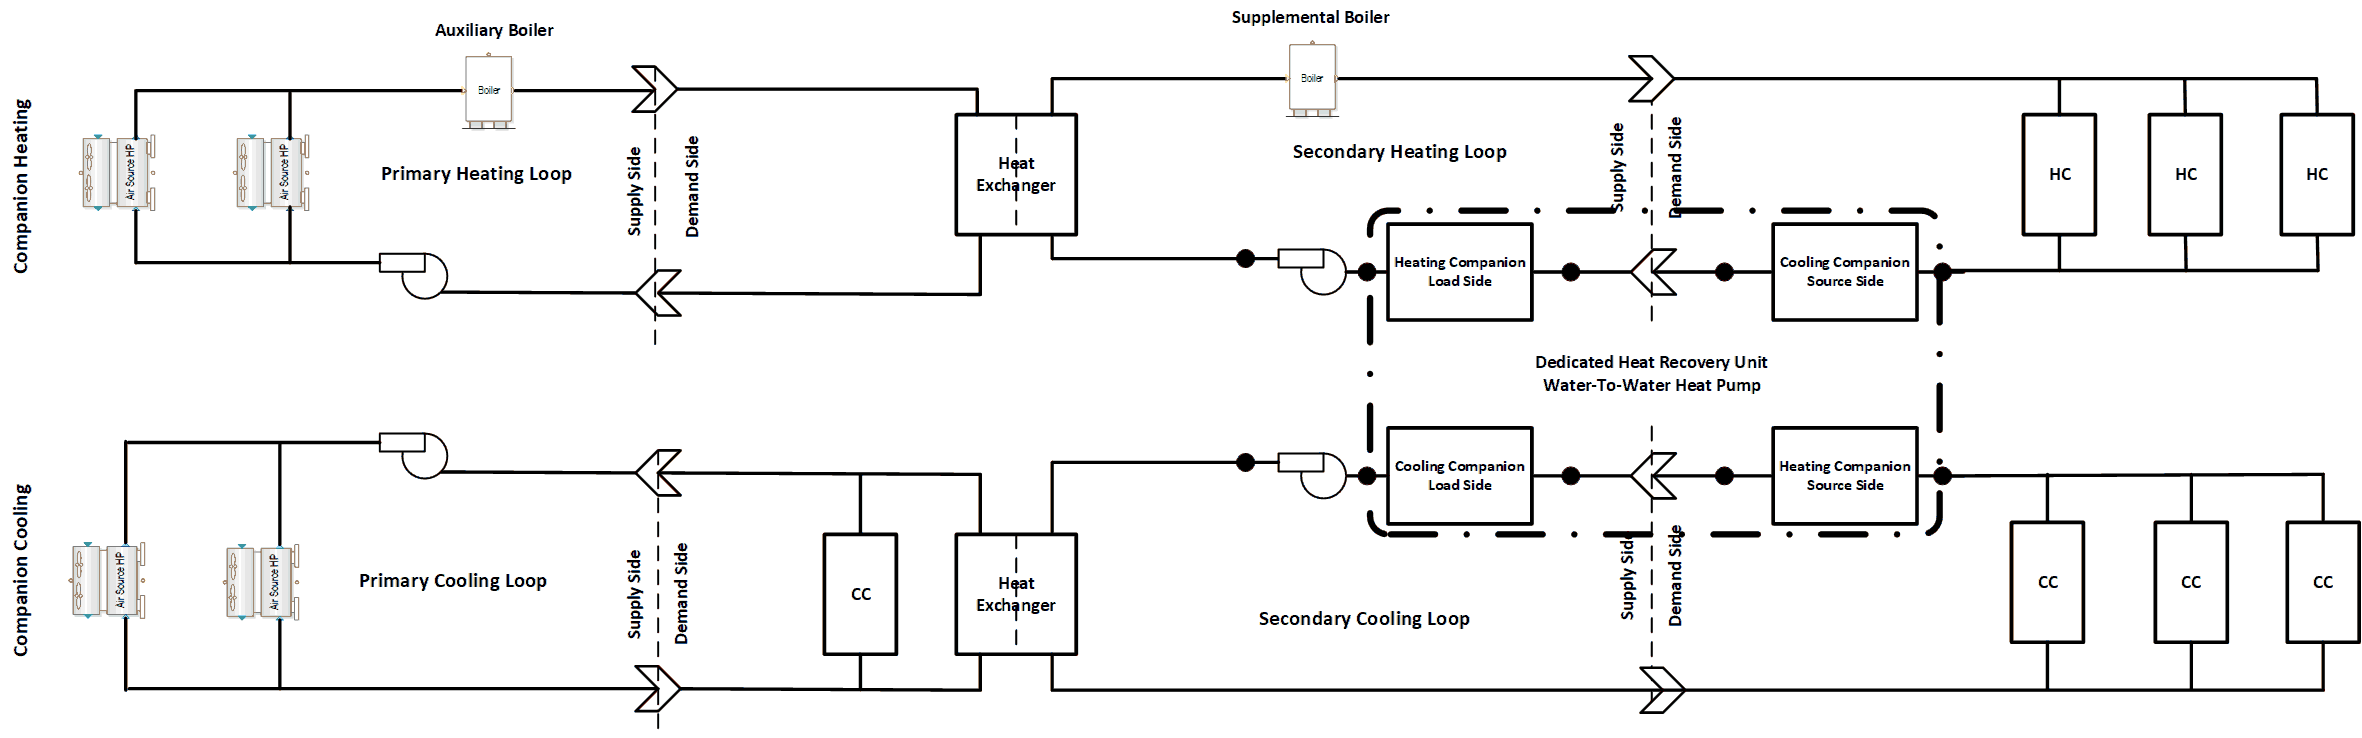
\includegraphics[width=1.0\textwidth, height=1.0\textheight, keepaspectratio=true]{media/ASHP_Plant.png}
\caption{Plant Configuration for Air Source Heat Pump Supervisory Control} \protect \label{fig:IO-ref-ASHP-Plant-Diag}
\end{figure}

This operation scheme also acts like a setpoint manager.  It calculates and applies setpoints to the outlet nodes of managed equipment, heat exchangers used for primary/secondary connections, boilers, and supply loop outlet nodes.  Traditional setpoint managers may be needed to get input past certain checks, but those are overwritten when using this supervisory plant controller.  The heat pumps are controlled by setting a temperature setpoint on the system node for the load side outlet node.  The setpoints for heating plants are adjusted using an outdoor air reset and control scheme.  The PlantLoop's input for the field called Load Distribution Scheme is not applied because the plant loads are not distributed explicitly, rather machines are turned on and off and setpoints are applied at the outlet of the heat pumps. The heating hydronic plant setpoints use a complex outdoor air reset scheme intended to serve air source heat pumps in heating mode where the supply temperature that the heat pump can deliver is constrained by the outdoor air temperature.  Then at very cold outdoor air conditions, the loop setpoint can be increased using a second stage backup outdoor air reset scheme. 

\begin{figure}[hbtp]
\centering
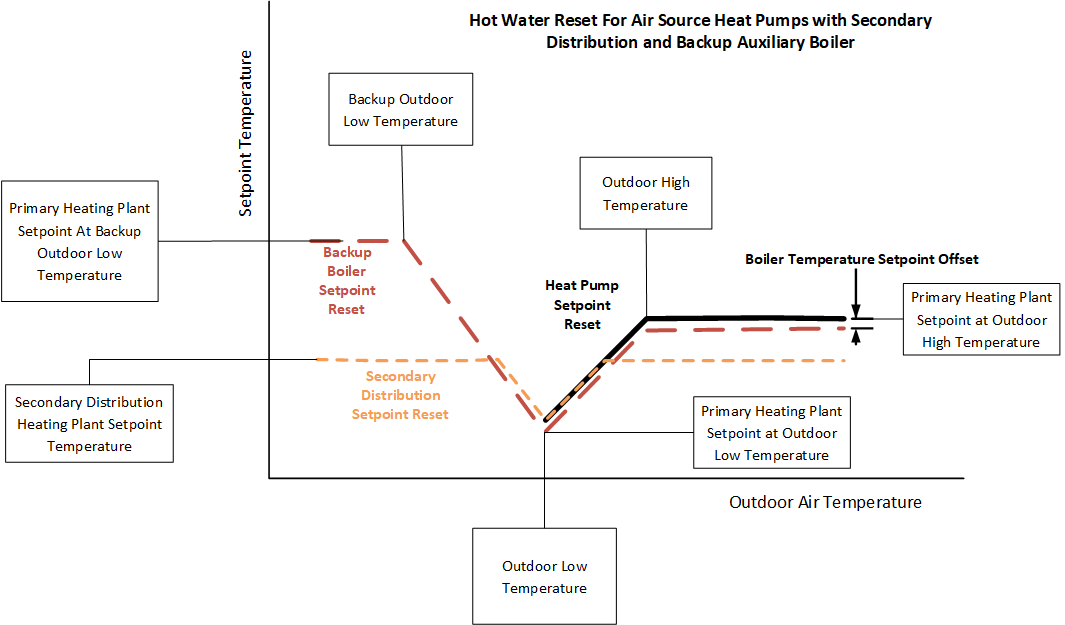
\includegraphics[width=0.9\textwidth, height=0.9\textheight, keepaspectratio=true]{media/HW_reset.png}
\caption{Hot Water Temperature Setpoint Vs Outdoor Air Temperature} \protect \label{fig:IO-ref-HW-reset-aux-backup-setpoint-reset}
\end{figure}

This plant operation scheme is unique in that the same instance of a PlantEquipmentOperation:ChillerHeaterChangeover is named in each of the plant loops being controlled.  So up to four plant loops will all use the same name of a PlantEquipmentOperation:ChillerHeaterChangeover as the scheme for that plant.  That is, each of the plant's PlantEquipmentOperationSchemes will list the same name for the PlantEquipmentOperation:ChillerHeaterChangeover.  It is expected there are two or four plant loops using the same operation scheme.  Two plants, one heating and cooling, are used if there is only simple primary loops and no secondary loops.  Four plants are expected for the most capabilities with both the heating system and the cooling system having primary/secondary loop arrangement (with a fluid to fluid heat exchanger connecting them).  For secondary loops, it is expected that a Sizing:Plant object is used and the input field called Loop Type is used to determine which loops are for heating and which are for cooling.  Even if the plant is hard sized, include a Sizing:Plant object so the routines can determine if a secondary loop is heating or cooling.  

This supervisory plant controller polls the building to see how the current loads favor operating the plants in either a cooling-only, heating-only, or simultaneous cooling and heating mode.  The building loads include the predicted sensible loads to setpoint for the listed zones, the ventilation loads on any central air handlers connected to those zones, and the loads from any process loads on plant (from a LoadProfile:Plant object).  The controller determines which of the three modes the plant should be in based on the polled building loads. 

Once the mode of operaton is determined, the controller dispatches the equipment based on the inputs for the operation scheme and equipment lists input for that mode using the current load on the primary plant side.  The heat pumps are modeled with companion objects, where a single machine has both cooling and heating input objects.  The PlantEquipmentOperation:CoolingLoad operating schemes should specify equipment lists with the cooling companion models (HeatPump:PlantLoop:EIR:Cooling) and the PlantEquipmentOperation:HeatingLoad operating schemes should point to the heating companion models (HeatPump:PlantLoop:EIR:Heating).  The heat pump model inputs need to set the Control Type to ``Setpoint'' control. 

This controller includes special handing of boiler backup.  Because air-source heat pumps can be limited in their ability to operate and cold outdoor air temperatures, in is necessary to coordinate boiler operation to provide heating during cold weather.  If a simple hot water boiler is present on the heating loops, it will be operated as a supplemental or auxilary heater to be used when the heat pumps cannot deliver.  For example when the outdoor air is below the Low Outdoor Air Temperature limit the air source heat pumps cannot operate and a boiler is used to meeting the setpoint.  Boilers found on a primary hot water loop are considered auxiliary boilers while boilers found on a secondary hot water loop are considered supplemental boilers.  Auxiliary boilers, if present, are operated when the outdoor air temperature is below the Outdoor Low Temperature and use the setpoint temperature determined by outdoor air reset.  The usual location of an auxiliary boiler is in the branch serving as the outlet branch on the supply side of the primary hot water loop.  Supplemental boilers, if present, are operated when the inlet fluid temperature is below a setpoint.  The setpoint is determined by the lower of the secondary hot water setpoint and the outdoor air reset.  The usual location of a supplemental boiler is in the branch serving as the outlet branch on the supply side of the secondary hot water loop.

This controller includes a special handling of a dedicated water to water heat pump used to recover heat directly between the return hot water and return chlled water.  The cooling and heating companions of this heat pump are named in the object.  These are used to efficiently exchange heat between the return flows on the secondary hot and chilled water returns.  This dedicated water to water heat pump will operate when there is sufficient flows in both returns and can be controlled to not operate when loads are high.  

\subsubsection{Inputs}\label{inputs-plantequipmentoperationchillerheaterchangeover}

\paragraph{Field: Name}\label{field-name-plantequipmentoperationchillerheaterchangeover}

This required alpha field contains the identifying name given to the PlantEquipmentOperation:ChillerHeaterChangeover object. This name is placed in the PlantLoop objects to select this scheme.  It is expected that both the heating and cooling plants will all point to this same operation scheme so that they can be controlled together. 

\paragraph{Field: Primary Cooling Plant Setpoint Temperature}\label{field-primary-chilled-water-temp-setpoint-plantequipmentoperationchillerheaterchangeover}

This required numeric field specifies the cooling plant operating setpoint temperature.  This is the primary chilled water plant loop.  The heat pumps in cooling mode will be operated to meet this setpoint. Degrees C.

\paragraph{Field: Secondary Distribution Cooling Plant Setpoint Temperature}\label{field-secondary-chilled-water-temp-setpoint-plantequipmentoperationchillerheaterchangeover}

This numeric field specifies the cooling plant operating setpoint for a secondary chilled water loop.  Degrees C. 

\paragraph{Field: Primary Heating Plant Setpoint at Outdoor High Temperature}\label{field-primary-hot-water-temp-setpoint-High-OA-plantequipmentoperationchillerheaterchangeover}

This required numeric field specifies the heating plant operating set point temperature at the high outdoor air temperature. Degrees C.

\paragraph{Field: Outdoor High Temperature}\label{field-hot-water-high-outdoor-air-temp-plantequipmentoperationchillerheaterchangeover}

This required numeric field specifies the high outdoor air temperature used for outdoor air reset and heat pump control.  Degrees C.

\paragraph{Field: Primary Heating Plant Setpoint at Outdoor Low Temperature}\label{field-hot-water-setpoint-reset-max-temp-diff-plantequipmentoperationchillerheaterchangeover}

This required numeric field specifies the heating plant operating set point temperature at the low outdoor air temperature. This value is generally set to the warmest temperature the heat pump can deliver at the Outdoor Low Temperature.  Degress C.

\paragraph{Field: Outdoor Low Temperature}\label{field-hot-water-setpoint-reset-ratio-plantequipmentoperationchillerheaterchangeover}

This required numeric field specifies the low outdoor air temperature used for outdoor air reset and heat pump control.  This serves as the lower limit for when air source heat pumps can operate in heaing mode.  If the outdoor air is colder than this setting, the air source heat pumps cannot operate.  Degrees C.

\paragraph{Field: Secondary Distribution Heating Plant Setpoint Temperature}\label{secondary-distribution-heating-plant-setpoint-temperature}

This numeric field specifies the heating plant operating setpoint for a secondary hot water loop.  Degrees C.  If the primary heating loop setpoint has been set below this as for outdoor air reset, then the secondary distribution loop may be set to the lower of this value and the outdoor air reset value. 

\paragraph{Field: Zone Load Polling ZoneList Name}\label{field-zone-load-polling-zonelist-name-plantequipmentoperationchillerheaterchangeover}

This alpha field specifies the ZoneList name that identifies each zone served by the hot and cold water plants. These zones are used to poll the current state of the building loads and are used to decide how the heat pump loops should be operated. 

\paragraph{Field: Cooling Only Load Plant Equipment Operation Cooling Load Name}\label{field-cool-only-load-equip-operation-name-plantequipmentoperationchillerheaterchangeover}

This alpha field specifies the PlantEquipmentOperation:CoolingLoad name that identifies the plant equipment and load ranges to meet a plant cooling load. This operation scheme is used when the supervisory control determines that the plants should be operated in a cool-only mode. 

\paragraph{Field: Heating Only Load Plant Equipment Operation Heating Load Name}\label{field-heat-only-load-equip-operation-name-plantequipmentoperationchillerheaterchangeover}

This alpha field specifies the PlantEquipmentOperation:HeatingLoad name that identifies the plant equipment and load ranges to meet a plant heating load. This operation scheme is used when the supervisory control determines that the plants should be operated in a heat-only mode. 

\paragraph{Field: Simultaneous Cooling And Heating Plant Equipment Operation Cooling Load Name}\label{field-simulataneous-cooling-and-heating-plant-equip-operation-cooling-name-plantequipmentoperationchillerheaterchangeover}

This alpha field specifies the PlantEquipmentOperation:CoolingLoad name that identifies the plant equipment and load ranges to meet a plant cooling load. When simultaneous heating and cooling plant loads exist at the same time, this equipment will be dispatched to meet the cooling plant load.

\paragraph{Field: Simultaneous Cooling And Heating Plant Equipment Operation Heating Load Name}\label{field-simulataneous-cooling-and-heating-plant-equip-operation-heating-name-plantequipmentoperationchillerheaterchangeover}

This alpha field specifies the PlantEquipmentOperation:HeatingLoad name that identifies the plant equipment and load ranges to meet a plant heating load. When simultaneous heating and cooling plant loads exist at the same time, this equipment will be dispatched to meet the heating plant load.

\paragraph{Field: Dedicated Chilled Water Return Recovery HeatPump Name}\label{field-dedicated-chilled-return-recovery-hp-name-plantequipmentoperationchillerheaterchangeover}

This alpha field specifies the name of a water-to-water heat pump (HeatPump:PlantLoop:EIR:Cooling) that connects its load side to the chilled water plant. This equipment will meet low loads on the chilled water plant while supplementing heating plant operation. It is expected the load side of this heat pump is located on the supply side of a secondary chilled water plant on the supply side inlet branch. The source side of this component is expected to be located on the demand side of a secondary hot water plant on the demand side outlet branch. This equipment may be switch off if chilled water plant loads are high depending on the load capacity factor set below.

\paragraph{Field: Dedicated Hot Water Return Recovery HeatPump Name}\label{field-dedicated-hot-return-recovery-hp-name-plantequipmentoperationchillerheaterchangeover}

This alpha field specifies the name of a water-to-water heat pump (HeatPump:PlantLoop:EIR:Heating) that connects its load side to the hot water plant. This equipment will meet low loads on the hot water plant while supplementing cooling plant operation. It is expected the load side of this heat pump is located on the supply side of a secondary hot water plant on the supply side inlet branch. The source side of this component is expected to be located on the demand side of a secondary chilled water plant on the demand side outlet branch. This equipment may be switch off if hot water plant loads are high depending on the load capacity factor set below.

Examples of this object:

\begin{lstlisting}

  PlantEquipmentOperation:ChillerHeaterChangeover,
    Two AWHP Operation Scheme , !- Name
    6.6 ,                                           !- Primary Cooling Plant Setpoint Temperature
    10.0,                                           !- Secondary Distribution Cooling Plant Setpoint Temperature
    59.8 ,                                          !- Primary Heating Plant Setpoint at Outdoor High Temperature
    10.0,                                           !- Outdoor High Temperature
    37.6 ,                                          !- Primary Heating Plant Setpoint at Outdoor Low Temperature
    0.0 ,                                           !- Outdoor Low Temperature
    45.0 ,                                          !- Secondary Distribution Heating Plant Setpoint Temperature
    All Conditioned Zones,                          !- Zone Load Polling ZoneList Name
    Two AWHP Cooling Operation Scheme,              !- Cooling Only Load Plant Equipment Operation Cooling Load Name
    Two AWHP Heating Operation Scheme,              !- Heating Only Load Plant Equipment Operation Heating Load Name
    One AWHP Cooling Operation Scheme,              !- Simultaneous Cooling And Heating Plant Equipment Operation Cooling Load Name
    One AWHP Heating Operation Scheme,              !- Simultaneous Cooling And Heating Plant Equipment Operation Heating Load Name
    Dedicated HR Cooling Side WSHP,                 !- Dedicated Chilled Water Return Recovery HeatPump Name
    Dedicated HR Heating Side WSHP;                 !- Dedicated Hot Water Return Recovery HeatPump Name

  ZoneList,
    All Conditioned Zones,         !- Name
    Basement,                         !- Zone name 1
    Core_bottom,                     !- Zone name 2
    Core_mid,                          !- Zone name 3
    continue with all zone names attached to these plant loops;

  PlantEquipmentOperation:CoolingLoad,
    Two AWHP Cooling Operation Scheme,  !- Name
    0.0,                                                   !- Load Range 1 Lower Limit {W}
    50000,                                               !- Load Range 1 Upper Limit {W}
    One AWHP Cooling Equipment List,        !- Range 1 Equipment List Name
    50000,                                               !- Load Range 2 Lower Limit {W}
    10000000000000,                                !- Load Range 2 Upper Limit {W}
    Two AWHP Cooling Equipment List;        !- Range 2 Equipment List Name

  PlantEquipmentList,
    Two AWHP Cooling Equipment List,  !- Name
    HeatPump:PlantLoop:EIR:Cooling,   !- Equipment 1 Object Type
    AWHP_1 Cooling Side,                   !- Equipment 1 Name
    HeatPump:PlantLoop:EIR:Cooling,   !- Equipment 2 Object Type
    AWHP_2 Cooling Side;                   !- Equipment 2 Name  
\end{lstlisting}

\paragraph{Output reporting available with the supervisory controller:}\label{operation-scheme-heating-outputs-description}

\begin{itemize}
    \item
    HVAC,Average,Supervisory Plant Heat Pump Operation Mode  {[}{]}
    \item
    HVAC,Average,Supervisory Plant Auxiliary Boiler Mode  {[}{]}
    \item
    HVAC,Average,Supervisory Plant Operation Polled Building Heating Load  {[}W{]}
    \item
    HVAC,Average,Supervisory Plant Operation Polled Building Cooling Load  {[}W{]}
    \item 
    HVAC,Average,Supervisory Plant Operation Primary Plant Heating Load  {[}W{]}
    \item
    HVAC,Average,Supervisory Plant Operation Primary Plant Cooling Load  {[}W{]}
    \item
    HVAC,Average,Supervisory Plant Heat Recovery Operation Mode  {[}{]}
    \item 
    HVAC,Average,Supervisory Plant Operation Secondary Plant Heating Load  {[}W{]}
    \item
    HVAC,Average,Supervisory Plant Operation Secondary Plant Cooling Load  {[}W{]}
\end{itemize}

\paragraph{Supervisory Plant Heat Pump Operation Mode}\label{operation-scheme-outputs-supervisory-plant-operation-mode}

This integer output represents the plant operating mode for the heat pumps as determined by the supervisory controller. Off = 0, Heating = 1, Cooling = 2 and Simultaneous Heating and Cooling = 3.This is the sum of the predicted zone sensible loads for the zones listed in the node list for this object, the ventilation loads on any central air systems connected to those zones, and the loads from any LoadProfile:Plant objects on the plant loops being supervised.



\paragraph{Supervisory Plant Auxiliary Boiler Mode}\label{operation-scheme-outputs-boiler-operation-mode}

This integer output represents the plant operating mode for the auxilary and/or supplemental boiler. Off = 0, Heating = 1.

\paragraph{Supervisory Plant Operation Polled Building Heating Load}\label{operation-scheme-outputs-supervisory-plant-operation-sensed-heating-load}

This numeric output represents the supervisory controller sensed building heating load in watts.  This is the sum of the predicted zone sensible loads for the zones listed in the node list for this object, the ventilation loads on any central air systems connected to those zones, and the loads from any LoadProfile:Plant objects on the plant loops being supervised. 

\paragraph{Supervisory Plant Operation Polled Building Cooling Load}\label{operation-scheme-outputs-supervisory-plant-operation-sensed-cooling-load}

This numeric output represents the supervisory controller sensed building cooling load in watts.  This is the sum of the predicted zone sensible loads for the zones listed in the node list for this object, the ventilation loads on any central air systems connected to those zones, and the loads from any LoadProfile:Plant objects on the plant loops being supervised. Cooling loads are negative values.

\paragraph{Supervisory Plant Operation Primary Plant Heating Load}\label{operation-scheme-outputs-supervisory-plant-heating-loads}

This numeric output represents the supervisory controller sensed loads on the primary plant heating loop in watts.

\paragraph{Supervisory Plant Operation Primary Plant Cooling Load}\label{operation-scheme-outputs-supervisory-plant-cooling-loads}

This numeric output represents the supervisory controller sensed loads on the primary plant cooling loop in watts.  Cooling loads are negative values.

\paragraph{Supervisory Plant Heat Recovery Operation Mode}\label{operation-scheme-outputs-hr-operation-mode}

This integer output represents the plant operating mode for the dedicated heat recovery water to water heat pump.  Off = 0, Heating led = 1, Cooling led = 2.  This output is only generated when the dedicated heat recovery option is used by naming the heating and cooling companions in the input object. 

\paragraph{Supervisory Plant Operation Secondary Plant Heating Load}\label{operation-scheme-outputs-supervisory-secondary-plant-heating-loads}

This numeric output represents the supervisory controller sensed loads on the secondary plant heating loop in watts.  This output is only generated when the dedicated heat recovery option is used by naming the heating and cooling companions in the input object. 

\paragraph{Supervisory Plant Operation Secondary Plant Cooling Load}\label{operation-scheme-outputs-supervisory-secondary-plant-cooling-loads}

This numeric output represents the supervisory controller sensed loads on the secondary plant cooling loop in watts.  Cooling loads are negative values. This output is only generated when the dedicated heat recovery option is used by naming the heating and cooling companions in the input object. 

\subsection{PlantEquipmentList}\label{plantequipmentlist}

\subsubsection{Inputs}\label{inputs-14-009}

\subsection{CondenserEquipmentList}\label{condenserequipmentlist}

The \hyperref[plantequipmentlist]{PlantEquipmentList} ~and CondenserEquipmentList ~specify available plant and condenser loop equipment respectively for any loop operation scheme. Each statement contains the object name, an identifying name (which links the definition back to one of the operation scheme statements) and a variable length of data pairs. These pairs refer to a plant equipment type and an identifying name. The type in this list of pairs must correspond to a valid plant object as described in the next subsection.

Note: If a \hyperref[plantequipmentlist]{PlantEquipmentList} or CondenserEquipmentList object is specified with no equipment object types or equipment names, then the corresponding PlantEquipmentOperation:* object will assume all available equipment on this plant (or condenser) loop should be OFF (not operate) within the specified lower/upper limit.

\subsubsection{Inputs}\label{inputs-15-009}

\paragraph{Field: Name}\label{field-name-8-013}

This alpha field contains the identifying name for the Equipment List.

\paragraph{Field Set: (Object Type, Name)}\label{field-set-object-type-name-1}

Remember the order of equipment on this list determines operation priority. Equipment on the list first will try to meet demand first. These fields tie to the Equipment Definition input structure, which must also be defined.

\paragraph{Field: Equipment \textless{}\#\textgreater{} Object Type}\label{field-equipment-object-type-1}

This alpha field contains the keyword for the type of equipment in operation. Example: (\hyperref[chillerelectric]{Chiller:Electric}, \hyperref[districtcooling]{DistrictCooling}). The full list of allowable plant equipment is valid plant objects as described in the next subsection.

\paragraph{Field: Equipment \textless{}\#\textgreater{} Name}\label{field-equipment-name-1}

This alpha field contains the identifying name for the equipment in operation. This distinguishes between two different pieces of equipment of the same type.

An example of this statement in an IDF is:

\begin{lstlisting}

PlantEquipmentList, Chiller Plant and Purchased,
          Chiller:Electric, Big Chiller,
          DistrictCooling, Purchased Cooling;
\end{lstlisting}

Note that this list is the middle range defined in the \hyperref[plantequipmentoperationcoolingload]{PlantEquipmentOperation:CoolingLoad} statement named ``Peak Operation'' above. This defines the equipment available when the load encountered by the plant (chiller water demand, for example) is between 7000 W and 24500 W. EnergyPlus will run the ``Big Chiller'' first up to its capacity and then attempt to meet the remaining load (while in that range) with the next piece of equipment (in this case, ``Purchased:Cooling'') in the list.